\section{Strumenti e strategie di versioning utilizzati}
In questa sezione vengono descritti gli strumenti e le strategie di versioning utilizzati durante lo sviluppo del progetto.

\subsection{Versioning System}
Come versioning system è stato utilizzato Git con hosting del repository su GitHub. Git è uno strumento che 
permette la collaborazione tra membri di un team che lavorano sul progetto tramite modifiche effettuate in 
locale, mediante clonazione del codice sorgente da parte di ognuno dei collaboratori, e una successiva 
congiunzione del lavoro sul repository remoto.
\\
\\
Repository su GitHub: \url{https://github.com/xFireFox27/BugBoard26-INGSW2526_015}

\begin{figure}[H]
        \centering
        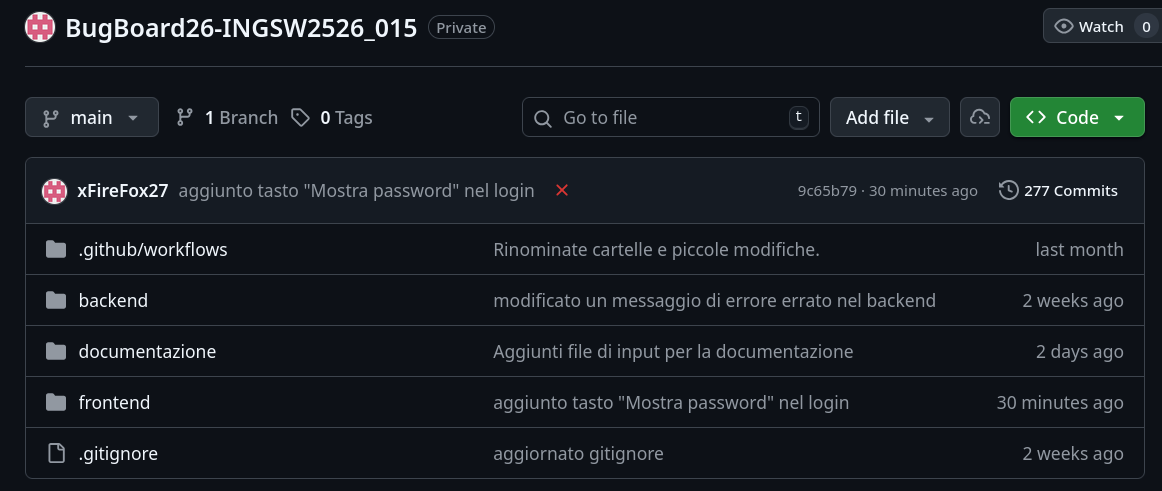
\includegraphics[width=1\linewidth]{src/descrizione-strumenti-versioning/Repository.png}
        \caption{Screenshoot del repository su GitHub}\label{ScreenshootRepo}
\end{figure}

\subsubsection{Branching Strategy}
Come branching strategy è stato utilizzato un "Centralized Workflow", una strategia che prevede che tutti i 
contributors lavorino direttamente sull'unico branch principale chiamato main. Questa strategia è quella 
che più facilmente si sposa con un gruppo ridotto di contributors a stretto contatto tra loro. 
In particolare le iterazioni prevedevano una comunicazione frequente tra i vari membri del team, 
con una divisione strategica dei task volta ad evitare overlap delle modifiche, limitando così errori 
derivanti dal merging, e l'incoraggiamento di commit frequenti per facilitare l'integrazione del codice e 
la rapida risoluzione di eventuali errori derivanti da conflitti. Questo tipo di strategia è perfetta per 
processi di sviluppo rapidi dato che taglia l'overhead derivante dalla gestione dei branch separati.

